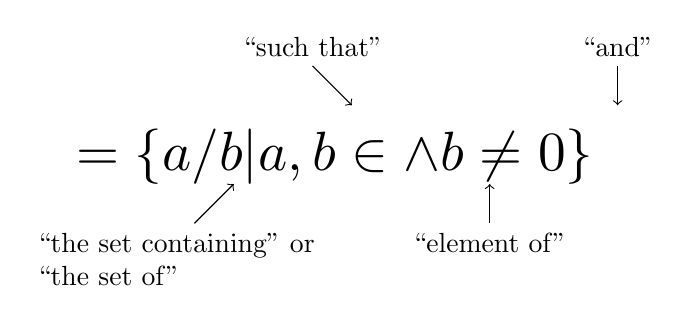
\begin{tikzpicture}
% equation
    \node[anchor=south west,scale=2] at (0,0) {\(\bbQ=\left\{a/b\middle|a,b\in\bbZ \wedge b\neq0\right\}\)};
% labels
    \draw[<-] (2.25,0.25) -- ++(-0.5,-0.5) node[anchor=north,text width=4cm]{``the set containing'' or ``the set of''};
    \draw[<-] (3.75,1.25) -- ++(-0.5,+0.5) node[anchor=south]{``such that''};
    \draw[<-] (5.5,0.25) -- ++(0,-0.5) node[anchor=north]{``element of''};
    \draw[<-] (7.125,1.25) -- ++(0,+0.5) node[anchor=south]{``and''};
% helper grid
    % \draw[red] (0,0) grid (10,2);
    % \draw[red,dashed,step=0.5] (0,0) grid (10,2);
\end{tikzpicture}
